\documentclass{../../text-style}

\texttitle{Лекция 7/Практика 6: Порождающие шаблоны}

\begin{document}

\maketitle
\thispagestyle{empty}

\section{Паттерн <<Фабричный метод>>}

\subsection{Мотивирующий пример}

Перейдём к порождающим паттернам. Допустим, мы хотим сделать игру-стратегию наподобие Age of Empires или Warcraft. У нас есть юниты: мечник, всадник и лучник. У них разные характеристики и разное поведение, но есть и много общего, и мы, естественно, хотим работать с ними единообразно, для чего заводим им общий базовый класс <<Warrior>>:

\begin{center}
    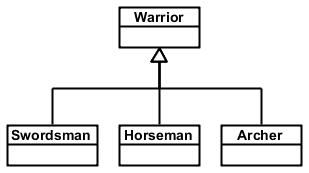
\includegraphics[width=0.4\textwidth]{warriors.png}
\end{center}

Теперь мы хотим реализовать класс <<Бараки>>, который будет производить юнитов, и, естественно, мы хотим написать содержательный код один раз, чтобы он работал со всеми типами юнитов. Однако проблема в том, что для вызова конструктора мы должны знать точный тип объекта --- виртуальных конструкторов не бывает, а в данном случае очень хочется. Не бывает не потому, что современные языки такие плохие, а потому, что в момент создания объекта определяется его тип времени выполнения, который как-то должен быть задан --- он и определяется конструктором, так что от вызова конструктора никуда не деться.

Однако если что-то очень хочется, народные умельцы найдут способ. Известен приём программирования, который называется <<Виртуальный конструктор>> (не делайте так, это плохая идея):

\begin{minted}{c++}
enum WarriorId { SwordsmanId, ArcherId, HorsemanId };

class Warrior
{
public:  
    Warrior(WarriorId id)
    {
        if (id == SwordsmanId) p = new Swordsman;
        else if (id == ArcherId) p = new Archer;
        else if (id == HorsemanId) p = new Horseman;
        else assert(false);
    }
    virtual void info() { p->info(); }
    virtual ~Warrior() { delete p;  p = 0; }
private:
    Warrior* p;
};
\end{minted}

В базовом классе Warrior заводится поле, которое будет указывать на реальный объект, и конструктор, который инициализирует это поле в зависимости от каких-то факторов (в нашем случае идентификатор требуемого типа юнита). Все запросы к объекту базового класса просто перенаправляются объекту <<настоящего>> класса (как info() в нашем примере). То есть Warrior, помимо того, что является базовым классом для конкретных юнитов, играет роль прокси, который позволяет выбрать реализацию, и даже при желании менять её во время выполнения. На диаграмме классов это выглядит как-то так:

\begin{center}
    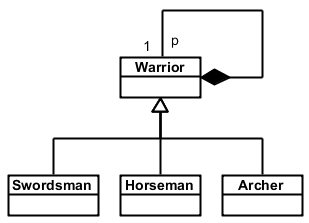
\includegraphics[width=0.35\textwidth]{warriorVirtualCtor.png}
\end{center}

Плохо это тем, что нарушается принцип единственности ответственности (Warrior слишком умный), добавляется ненужный уровень косвенности (и затраты на вызовы методов через прокси), и для каждого юнита хранится два комплекта полей Warrior, один из которых не используется (один в прокси, другой в проксируемом объекте, который наследуется от Warrior), да ещё и Warrior больше нельзя сделать абстрактным.

Можно улучшить эту идею, заменив извращённый конструктор на статический метод (делайте так иногда, это адекватный, хотя и не всегда лучший способ решения проблемы):

\begin{center}
    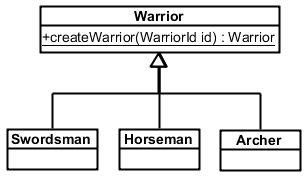
\includegraphics[width=0.35\textwidth]{warriorFactoryMethod.png}
\end{center}

Метод createWarrior всё так же содержит выбор конструктора и всё так же хочет знать, кого ему создавать, поэтому принимает id. Но по крайней мере Warrior можно оставить абстрактным и нет никаких проблем с вызовами через прокси (правда, мы теперь во время выполнения не можем поменять тип юнита, но это обычно и не надо, а если будет надо, можно сделать более явным образом).

\subsection{Фабричный метод (Factory Method), общая структура}

Следующий шаг развития идей модельного примера приведёт нас уже к настоящему фабричному методу: сделать метод создания не статическим, а виртуальным, и заменить цепочку if-ов на вызов виртуального метода. На диаграмме классов это выглядит так:

\begin{center}
    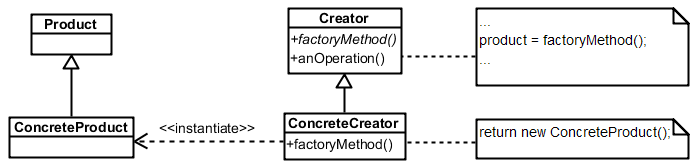
\includegraphics[width=0.9\textwidth]{factoryMethod.png}
\end{center}

Creator --- это класс, которому надо создать объект, но он заранее не знает, какого тот типа. Тогда Creator может объявить себе абстрактный метод factoryMethod (тот самый фабричный метод, в честь которого назван паттерн), и дальше пользователи Creator-а могут унаследоваться от него, переопределив этот factoryMethod так, чтобы он возвращал нужный объект. Обычно его реализация пишется в одну строчку и сводится к вызову конструктора. Product --- это общий интерфейс всех возможных продуктов, он является типом возвращаемого значения factoryMethod. ConcreteProduct-ов может быть сколько угодно, для каждого из них надо будет объявить ConcreteCreator, чтобы тот его создавал и тем самым параметризовал Creator подклассом Product-а.

Кажется, что это может понадобиться очень редко, но на самом деле паттерн применяется весьма  часто, в ситуациях, когда Creator делает много содержательной работы, но часть её делегирует Product-у, и Product может делать эту работу по-разному (например, <<Фабричный метод>> может создавать стратегию для паттерна <<Стратегия>>, где Creator будет играть роль Context-а). Это на самом деле очень удобный способ параметризовать один объект другим объектом, не передавая его явно извне (например потому, что объект должен создавать Product-ы в больших количествах и по ходу работы).

В примере со стратегией Product-ом был бы Warrior, ConcreteProduct-ами были бы Archer, Swordsman и Horseman, а Creator-ом --- бараки, которые могли бы быть уточнены подклассами <<Бараки мечников>>, <<Поле для лучников>> и <<Конюшни>>. Каждый подкласс реализовывался бы в одну строку, что несколько неуклюже, но решает нашу проблему с переиспользованием кода бараков для разных типов юнитов. Вот ещё пример, из книги Банды Четырёх:

\begin{center}
    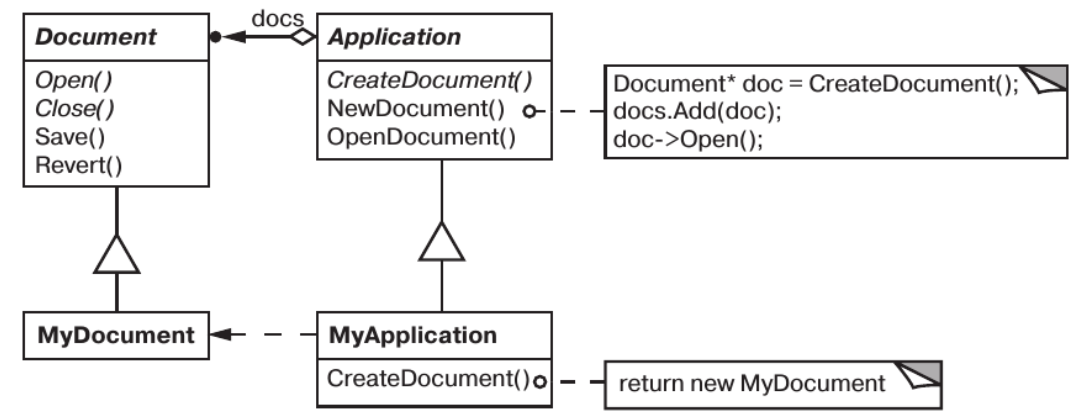
\includegraphics[width=0.85\textwidth]{factoryMethodForTextEditor.png}
\end{center}

Тут речь идёт о фреймворке, который позволяет создавать редакторы разных форматов файлов (например, текстовых и изображений). Есть абстрактный базовый класс Document, от которого мы должны отнаследоваться, чтобы реализовать свой формат, и абстрактный класс Application, в котором делается много содержательной работы (типа открытия и создания документа). От него мы должны унаследоваться и переопределить фабричный метод CreateDocument(), чтобы он возвращал наш вид документов, всё остальное фреймворк сделает сам. 

\subsection{Детали реализации}

 Creator на самом деле вовсе не обязан быть абстрактным --- он вполне может предоставлять реализацию фабричного метода по умолчанию. Это может быть полезно, если фабричный метод является на самом деле точкой расширения на будущее --- пользователи Creator могут переопределить создаваемый объект, но не обязаны это делать. Это же и минус такого подхода --- пользователи могут забыть переопределить фабричный метод и получить внезапное поведение по умолчанию, а не ошибку компиляции.

 Фабричный метод вполне может принимать параметры и даже выбирать в зависимости от них тип создаваемого объекта. 
 
 Если язык поддерживает инстанцирование по прототипу (например, JavaScript или Smalltalk), можно ничего и не выбирать, и даже не наследовать конкретный Creator --- просто параметризуем Creator прототипом и делаем его клон при необходимости.

 Маленькая тонкость, про которую, тем не менее, надо помнить --- Creator не может вызывать фабричный метод в конструкторе, так что если хочется параметризовать действия, совершаемые в конструкторе, придётся использовать что-то ещё. Почему --- в момент вызова конструктора предка (Creator) конструктор потомка (ConcreteCreator) ещё не отработал и потомок находится в неконсистентном состоянии. Вызов любого виртуального метода в конструкторе предка, не только фабричного метода, приведёт либо к ошибке компиляции, либо, что гораздо хуже, к внезапным и трудноотлаживаемым ошибкам времени выполнения.

 Один из способов решения этой проблемы --- если язык позволяет, заменить наследование параметризацией шаблона (как мы уже делали в паттерне <<Стратегия>>). В Java это работать не будет, создать объект типа-параметра шаблона там нельзя. В C\# и C++ это вполне валидная альтернатива классической реализации.

 Ну и конечно, вместо фабричного метода можно использовать лямбда-функцию, которая будет по требованию создавать Product-ы, и передавать её Creator-у при инициализации. В современных языках это, пожалуй, лучший на самом деле способ реализации этого паттерна, который в Книжке не описан --- в те времена, когда она писалась (и даже когда выходили её переиздания), лямбда-функций в нормальных языках ещё не было.

\section{Паттерн <<Абстрактная фабрика>>}

\subsection{Мотивирующий пример}

Вернёмся к текстовому редактору, на примере которого рассказывалось большинство паттернов. Теперь наша задача --- поддержать разные стили оформления пользовательского интерфейса. Нам хочется иметь возможность выбирать стиль при запуске редактора. Например, если запустили под Windows, используется внешний вид элементов, типичный для Windows, если под Linux, то внешний вид, типичный для местного оконного менеджера (В Java AWT, кстати, была такая функциональность). И хочется иметь возможность удобно расширять набор стилей (хотя бы потому, что оконных менеджеров под Linux очень много). Поэтому мы начнём с того, что реализуем абстрактные элементы и конкретные реализации под каждый из пока поддерживаемых стилей:

\begin{center}
    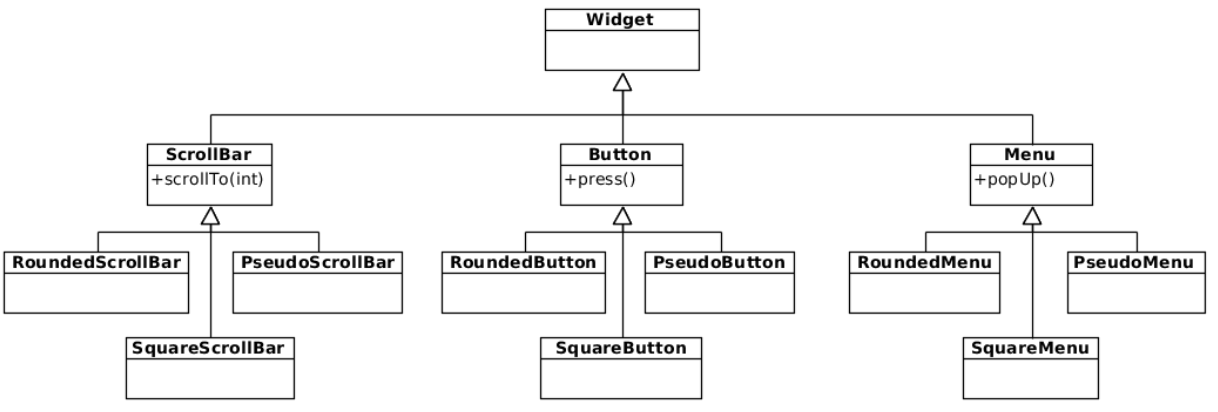
\includegraphics[width=0.9\textwidth]{widgets.png}
\end{center}

Очень напоминает ситуацию в паттерне <<Мост>> до рефакторинга, и кажется, что можно избежать квадратичного числа классов, но тут ничего не выйдет --- разные элементы управления должны реально выглядеть по-разному, и там должен быть какой-то произвольный код, который никуда из них не вынести. Поэтому будем жить с этим.

Проблема возникает в том, как эту иерархию использовать в коде редактора. Наивный подход --- при создании каждого окна смотреть, какой стиль используется, и в зависимости от этого создавать те или иные конкретные элементы управления, --- упирается в то, что окон в редакторе может быть очень много, и если в каждом написать гигантский switch, нам быстро надоест. И добавление нового стиля превратится в пытку, с тысячей ошибок времени выполнения, когда мы где-то забыли добавить вариант.

Поэтому предлагается вынести код создания объектов в отдельный класс, и использовать его везде, где надо создавать объект. Например, если нам надо создать полосу прокрутки, мы пишем не \mintinline{c++}|ScrollBar* bar = new RoundedScrollBar;|, а \mintinline{c++}|ScrollBar* bar = guiFactory->createScrollBar();|. Гигантский switch можно в таком случае реализовать в guiFactory, и передавать её везде, где надо создавать элементы --- это позволит при добавлении нового стиля поменять только одно место в коде, и избежать копипаста. А можно вспомнить, что если у вас где-то есть гигантский switch, то вы можете переделать его в вызов виртуальной функции, и получить уже настоящий паттерн <<Абстрактная фабрика>>:

\begin{center}
    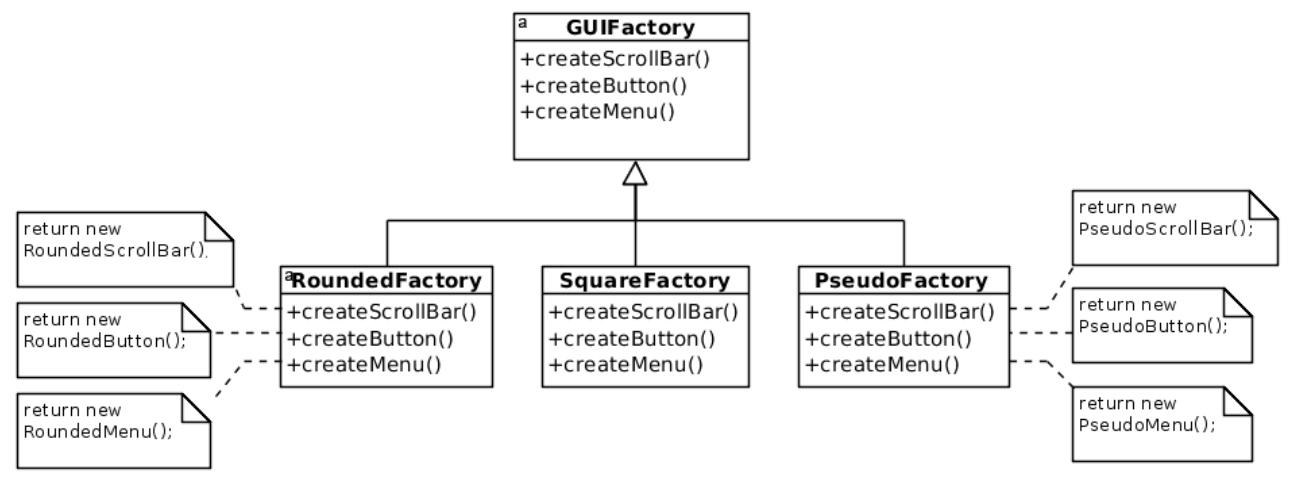
\includegraphics[width=0.95\textwidth]{widgetFactory.png}
\end{center}

Один гигантский switch нам всё-таки будет нужен --- при старте приложения мы смотрим, какой визуальный стиль нам нужен, и выбираем, какую фабрику создать. Дальше отдаём эту фабрику всем, кто планирует создавать элементы управления, они запрашивают у неё элемент, она возвращает нужный. Каждая фабрика --- это набор однострочных методов, которые просто вызывают конструктор нужного типа.

\subsection{Абстрактная фабрика (Abstract Factory), общая структура}

Эта идея обобщается до следующей схемы:

\begin{center}
    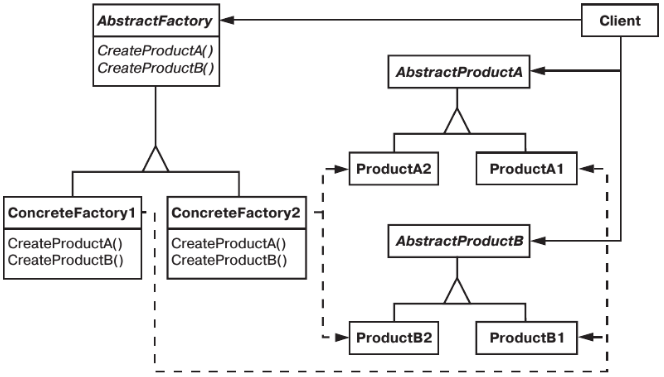
\includegraphics[width=0.7\textwidth]{abstractFactory.png}
\end{center}

Есть набор продуктов (в нашем примере --- разных элементов управления), продукты образуют иерархии, но разные типы продуктов могут быть никак не связаны друг с другом. Есть абстрактная фабрика, декларирующая умение создавать абстрактные продукты, и наследующиеся от неё конкретные фабрики, каждая из которых умеет создавать свой вид конкретного продукта каждого типа. Клиент, желающий создавать продукты, знает только про абстрактные продукты и про абстрактную фабрику. Кто-то ещё должен уметь создать конкретную фабрику --- либо сам клиент, либо кто-то ещё, и отдать её клиенту.

Это позволяет очень хорошо изолировать конкретные классы от тех мест, где они будут использоваться --- клиент знает только про абстракции (которые, скорее всего, просто интерфейсы), а конкретные продукты ему могут быть не видны вообще, и даже не быть доступны во время компиляции клиента (например, подключаться в виде плагина). Чтобы подменить вид продуктов, достаточно просто передать клиенту новую фабрику. Единственное, что клиент уже мог успеть насоздавать продуктов, поэтому если хочется изменить вид продуктов уже после инициализации клиента, надо делать механизм, позволяющий его переинициализировать (что как правило хлопотно, поэтому многие приложения просят себя перезапустить после столь радикальных изменений).

При этом, правда, добавление нового типа продуктов (то есть AbstractProductC) довольно хлопотно, придётся в каждую существующую фабрику добавить новый метод, и поправить код клиента, чтобы он им пользовался. Добавление нового вида продукта (то есть ProductA3,  ProductB3 и т.д.) требует добавления новой фабрики, что обычно гораздо проще. Кстати, наличие общего интерфейса у каждого типа продукта гарантирует их совместимость, то есть при добавлении нового продукта он гарантированно будет вести себя как все остальные --- это бесплатный бонус при использовании паттерна <<Абстрактная фабрика>>.

Применяется абстрактная фабрика в следующих ситуациях (достаточно истинности одного условия, чтобы задуматься о применении паттерна):

\begin{itemize}
    \item система не должна зависеть от того, как создаются входящие в неё объекты: если мы хотим создать один объект, то это не страшно, а вот если продукт требует инициализации здоровенной подсистемы, логику инициализации может иметь смысл вынести в фабрику просто для того, чтобы спрятать её от клиента;
    \item система должна конфигурироваться типом объектов, с которыми она будет работать --- это всяческая поддержка стилей, вариантов реализации (например, в примере с роботами из паттерна <<Мост>> фабрика могла создавать объекты для управления конкретным типом робота), поддержка плагинов;
    \item взаимосвязанные объекты должны использоваться вместе --- фабрика не даст перепутать и создать все кнопки в стиле Windows, кроме одной;
    \item хотите предоставить библиотеку объектов, раскрывая только их интерфейсы, но не реализацию --- тогда создать объекты с помощью конструкторов у клиента физически не выйдет, фабрика будет играть роль этакой библиотеки конструкторов, через которую клиент и будет получать объекты.
\end{itemize}

Фабрику можно рассматривать как класс, состоящий из нескольких реализаций паттерна <<Фабричный метод>>. Принципиальное отличие в том, что в паттерне <<Фабричный метод>> предполагается, что класс, где этот самый фабричный метод находится, сам делает массу содержательной работы и использует фабричный метод только для дополнительного конфигурирования. <<Абстрактная фабрика>> же --- это выделенный класс, цель существования которого --- только создание объектов и ничего больше.

\subsection{Детали реализации}

Абстрактная фабрика хорошо комбинируется с паттерном <<Одиночка>>, который мы рассмотрим следующим. Скорее всего, фабрика одна на всю систему, и вместо того, чтобы старательно передавать её всюду, где она нужна, можно сделать её доступной глобально. Однако в обсуждении паттерна <<Одиночка>> мы рассмотрим, почему это может быть плохой идеей, так что пользоваться таким приёмом надо с большой осторожностью.

Если типов продуктов много, то можно рассмотреть возможность не создавать кучу подклассов абстрактной фабрики, а сделать <<универсальную>> фабрику, которая во время выполнения параметризуется создаваемыми продуктами. Для этого можно использовать паттерн <<Прототип>> (про который чуть позже), тем более если в языке реализации так принято (например, JavaScript). А можно параметризовать фабрику лямбда-функциями, которые будут создавать объект. А можно, если язык позволяет, сделать фабрику шаблоном и конкретные типы передавать при инстанцировании шаблона как параметры-типы (но это куда как страшнее, чем использование аналогичного приёма в паттерне <<Стратегия>>, потому что типов продуктов обычно много и параметров шаблона будет тоже много --- поэтому не разу не встречал такого способа на практике). А ещё можно использовать рефлексию и параметризовать фабрику объектами-типами (например, Class в Java или Type в .NET), из которых с помощью рефлексии создавать продукты, но не нужно --- использовать рефлексию без нужды всегда плохая идея.

Ещё методы создания объектов в фабрике могут принимать параметры, исходя из которых выбирать, объект какого типа они хотят создать. Однако, в отличие от аналогичного приёма в паттерне <<Фабричный метод>>, это может сильно запутать дело. Есть соблазн с помощью параметра выбирать одно из семейств (например, вместо CreateScrollBar и CreateButton сделать метод CreateWidget, принимающий, что за элемент управления надо создать), но это очень рискованная идея, потому что нарушается типобезопасность --- клиент без идей, продукт какого типа ему вернули, и компилятор не может проверить, что правильного.

\section{Паттерн <<Прототип>>}

\subsection{Мотивирующий пример}

Положим, мы теперь разрабатываем редактор нотной записи. Там есть нотный стан, на который надо уметь из палитры вытаскивать ноты разных длительностей. Хочется иметь возможность легко расширять палитру и не писать произвольный код создания каждого вида нот в гигантском switch при начале операции drag-and-drop. Можно снабдить палитру кучей фабрик, но есть более элегантное решение, которое, к тому же, позволит нам легко копировать уже существующие части нотной записи. Мы сделаем всем объектам, которые могут быть на нотном стане, метод Clone(), и в палитру добавим прототипы этих объектов --- то есть по одному объекту каждого типа, которые можно будет клонировать и тащить на нотный стан:

\begin{center}
    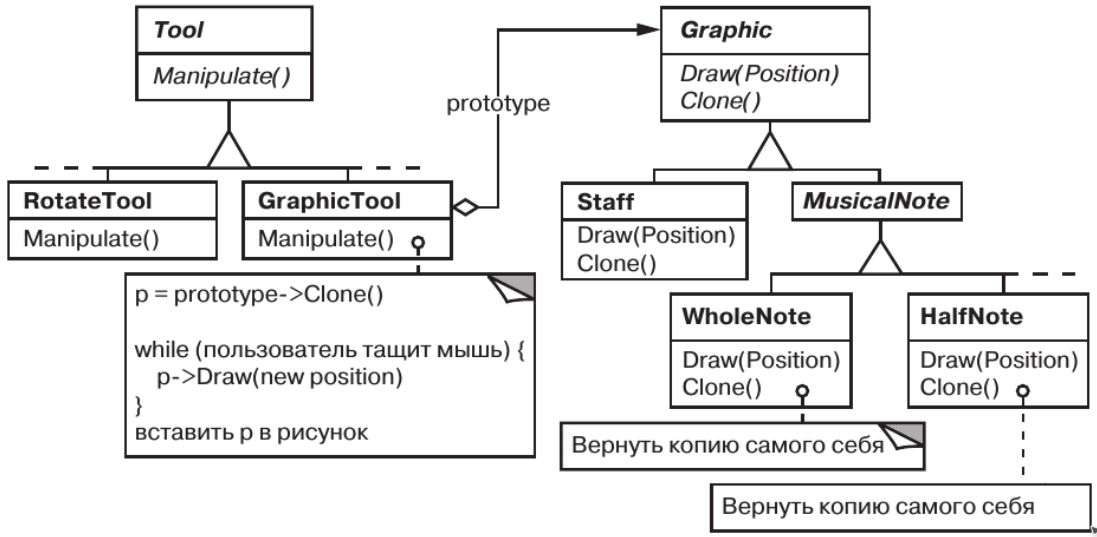
\includegraphics[width=0.9\textwidth]{musicalEditor.png}
\end{center}

Класс Graphic --- общий базовый класс (или интерфейс) для всего, что есть в палитре и на нотном стане, он декларирует возможность рисовать элемент и клонировать элемент, порождая его точную копию. GraphicTool --- это клиент Graphic, он реализует операции над элементами, в частности, drag-and-drop. При клике мышью на палитре он вызывает Clone() элемента палитры, на который кликнули, тот создаёт ему копию себя, которую и тащат на нотный стан.

\subsection{Прототип (Prototype), общая структура}

Обобщается идея до паттерна <<Прототип>> с вот такой, по сути очень простой, структурой:

\begin{center}
    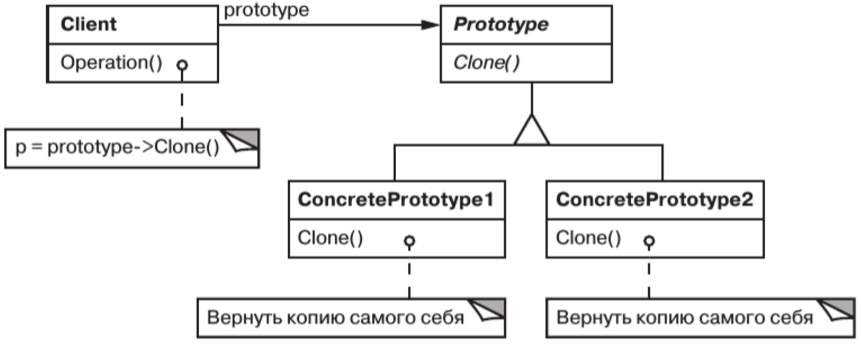
\includegraphics[width=0.8\textwidth]{prototype.png}
\end{center}

Фактически весь паттерн сводится к тому, что декларируется метод Clone() и предлагается использовать его для порождения копий нужных объектов. Обратите внимание, что это тоже помогает устроить что-то вроде виртуального конструктора: Clone() виртуальный, и создаёт копию объекта того класса, от которого он в итоге вызвался --- клиент про тип объекта ничего не знает.

\subsection{Детали реализации}

Прототип можно реализовать через рефлексию, если она поддерживается в языке. Вытащить тип времени выполнения и запустить его конструктор рефлексией вполне можно, и даже скопировать значения полей. Но, как обычно, рефлексией стоит пользоваться только если очень надо, тут может быть проще и лучше самим Clone() реализовать.

Прототип обычно полезен не сам по себе, а с каким-то способом быстро получить нужный прототип. В примере про музыкальный редактор это делала палитра, определяя по координатам клика мышью, какой элемент надо создать. Иногда применяют реестр прототипов --- ассоциативное хранилище (быть может, <<Одиночка>>), где можно легко найти и клонировать нужный объект.

Самое хитрое в паттерне --- это реализация Clone(). Во-первых, надо ответить себе на вопрос, хотим ли мы глубокое или мелкое копирование:

\begin{itemize}
    \item глубокое копирование копирует объект, объекты, на которые он ссылается, объекты, на которые ссылаются они, и т.д., то есть весь граф по ссылкам;
    \item мелкое копирование копирует только сам объект, оставляя ссылки такими, какие они были.
\end{itemize}

Глубокое копирование --- это то, что ожидается любыми нормальными людьми, поэтому если нет веских причин поступить иначе, надо, чтобы Clone() выполнял именно его. Однако реализовать глубокое копирование, особенно если в графе копируемого объекта есть круговые ссылки, может быть довольно нетривиально --- надо делать честный обход, запоминать ссылки на уже скопированные объекты и т.д. И работать это, естественно, будет гораздо дольше, чем мелкое копирование, особенно если граф объектов большой. И мелкое копирование вполне можно использовать, если вся структура немутабельна и от разделения объектов никому плохо не будет.

Немного хакерский способ быстро реализовать глубокое копирование --- взять объект, сериализовать его с помощью какой-нибудь библиотеки сериализации (в память, естественно, не на диск), а потом десериализовать. Тут, правда, надо следить за идентичностью результата --- например, если в объекте был какой-то id-шник, то библиотека сериализации скопирует его как он есть, и мы получим два разных объекта с одним id-шником, что наверняка закончится трагедией. Однако никто не мешает все поля, которые у оригинала и у клона должны быть разными, подправить после клонирования руками. Почему способ хакерский --- потому что это быстро и просто реализовать, но работать будет заведомо медленнее, чем реализация Clone() вручную. Так что в продакшн-коде так лучше не делать.

Ещё один тонкий момент --- это если в клоне должны быть ещё какие-то, кроме идентификатора, значения, отличные от оригинала. Возникает соблазн сделать методу Clone() параметры, которыми можно было бы проинициализировать созданный клон, однако если посмотреть на стандартные библиотеки, где этот паттерн реализован, никто так не делает. Clone() не принимает параметры неспроста --- каждому конкретному прототипу для инициализации, скорее всего, потребуется свой набор параметров (не сейчас, так в будущем). Ну а объявить Clone() в базовом классе, просто объединив множества всех нужных параметров --- очень неООПшно и хрупко (придётся менять интерфейс каждый раз, когда у кого-то из подклассов меняется какой-то параметр).

\section{Паттерн <<Строитель>>}

\subsection{Мотивирующий пример}

Начнём с одного порождающего паттерна, который не поместился в предыдущую лекцию. Предположим, мы хотим сделать утилиту, которая бы читала текст в некотором формате (допустим, .rtf) и конвертировала бы его в другой формат (например, TeX, .docx, plain text и т.д.). .rtf содержит информацию о структуре текста и его форматировании. Мы не хотим писать несколько разных конвертеров, а хотим считать .rtf один раз и конвертировать его в разные целевые форматы, причём не строя какого-то внутреннего представления (поскольку формат довольно простой и усложнять систему не хотелось бы).

На помощь приходит паттерн <<Строитель>>:

\begin{center}
    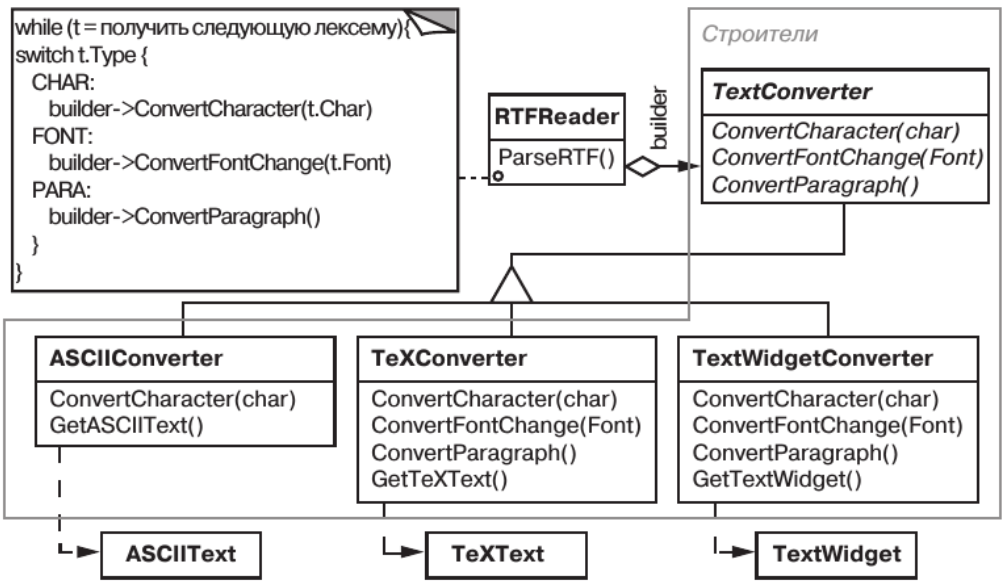
\includegraphics[width=0.9\textwidth]{textConverter.png}
    \attribution{Э. Гамма и др., Приемы объектно-ориентированного проектирования}
\end{center}

Есть класс RTFReader, который занимается разбором .rtf-документа. Он параметризуется одним из видов конвертеров, каждый из которых принимает элементы документы и что-то с ним делает. Например, ASCIIConverter может просто каждый переданный символ добавлять к строке, а команды форматирования просто игнорировать. Задача RTFReader --- последовательно <<скормить>> весь документ установленному в него конвертеру. Забрать результат потом можно с помощью метода Get-что-то-там у конвертера (они у всех разные).

Теперь, во-первых, процесс конвертации строго детерминирован и управляется централизованно в RTFReader, во-вторых, конвертеры легко менять, поскольку они реализуют один интерфейс и RTFReader-у всё равно, с кем из них работать. И реализовывать конвертеры просто, поскольку им не надо заботиться о разборе документа, и пони получают документ маленькими частями.

\subsection{Строитель (Builder), общая структура}

Эта идея обобщается до паттерна <<Строитель>>:

\begin{center}
    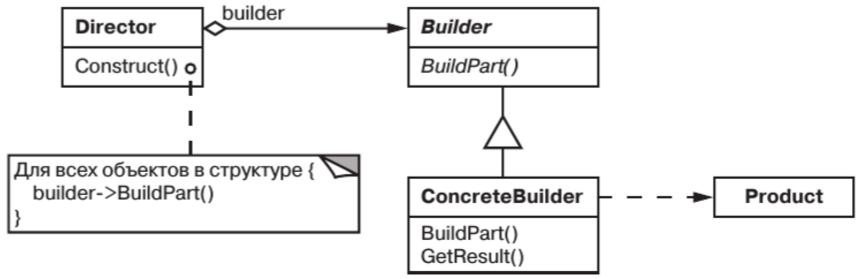
\includegraphics[width=0.85\textwidth]{builder.png}
    \attribution{Э. Гамма и др., Приемы объектно-ориентированного проектирования}
\end{center}

Класс Director (<<распорядитель>> в русскоязычной литературе) параметризуется Builder-ом и отвечает за то, чтобы передавать Buider-у части строящегося объекта (RTFReader в нашем примере). Builder --- интерфейс или абстрактный класс, имеющий методы, принимающие разные виды частей. Конкретный Builder реализует интерфейс Builder-а и постепенно строит Product. Когда процесс закончен, тот, кто заказывал строительство (Director или тот, кто создал Director и Builder), может получить Product с помощью метода GetResult().

\subsection{Детали реализации}

В реализации самое важное --- это определить интерфейс Builder так, чтобы любой конкретный строитель получал все необходимые части и мог эффективно строить Product. Обратите внимание, что GetResult() не является частью интерфейса Builder, и это важно по следующим причинам:

\begin{itemize}
    \item разные ConcreteBuilder-ы могут строить разные Product-ы, никак не связанные иерархией наследования;
    \item Director-у не нужно знать про продукты вовсе, он просто обходит структуру и отдаёт её части Builred-у; что именно строится, его не волнует;
    \item помимо Director и Builder, по всей видимости, где-то есть клиент, который и заказывает стройку --- клиент создаёт Builder, создаёт Director, передавая ему Builder, и запускает Construct() у Director-а. По окончании строительства у клиента всё ещё есть ссылка на конкретный Builder, потому что он же его и создал. Соответственно, клиент может забрать результат, вызвав GetResult().
\end{itemize}

Ещё иногда стоит Builder делать всё-таки абстрактным классом, а не интерфейсом, чтобы сделать его методам пустые реализации по умолчанию\footnote{Недавно в современных языках возникла мода на реализации по умолчанию для методов интерфейсов --- изначально это появилось в Java как средство обеспечения обратной совместимости при расширении интерфейсов (код, который не знает про новые методы интерфейса, может благодаря реализации по умолчанию их не реализовывать, соответственно, не надо перекомпилировать миллионы строк кода). Потом этот механизм начали неправильно использовать, и вот, интерфейс и абстрактный класс теперь почти неотличимы.}. Это мы использовали в мотивирующем примере для реализации ASCIIConverter-а, которому большая часть тегов RTF-документа (относящихся к форматированию) не интересна в силу природы конструируемого объекта.

В реальной жизни паттерн <<Строитель>> встречается довольно часто --- например, в любой нормальной стандартной библиотеке есть класс StringBuilder или его аналоги. Это класс, нужный для конкатенации нескольких строк в одну. Наивное решение:

\begin{minted}{csharp}
    var result = ""
    foreach (var string in stringList) {
        result += string;
    }
\end{minted}

Оно на самом деле квадратично по времени и по памяти, хотя выглядит линейным. Дело в том, что при каждой конкатенации выделяется память под хранение результирующей строки и обе конкатенируемые строки копируются в выделенную область. Потом сборщик мусора может подчистить промежуточные результаты, но это тоже занимает кучу времени. Если мы хотим сконкатенировать тысячу коротких строк, делать так --- очень плохая идея.

На помощь приходит StringBuilder. У него есть метод, позволяющий добавить строку к списку конкатенируемых строк, и метод, позволяющий получить результат. Добавление строки просто кладёт её в список, за константное время. Получение результата --- это пробежаться по списку, узнать длины всех строк, сложить (за линейное относительно количества строк время), сделать \emph{одно} выделение памяти для хранения результата, и скопировать туда последовательно строки из списка (за линейное относительно количества символов время).

В этом примере StringBuilder --- это, очевидно, Builder, а код, который его использует, выступает в роли и Director-а, и клиента одновременно.

Второй пример --- это подсистема работы с графами известной библиотеки Guava\footnote{Если вы знакомы с C++, Guava для Java --- примерно как Boost для C++. Страница Google Guava на GitHub: \url{https://github.com/google/guava} (дата обращения: 28.08.2021г).}. Там графы бывают трёх видов: Graph (граф в классическом математическом понимании, множество узлов и бинарное отношение на этом множестве, представляющее рёбра), ValueGraph (граф с метками на рёбрах) и Network --- то, что у нас обычно называют мультиграфом (или псевдографом): граф с параллельными рёбрами (то есть где ребро не просто элемент отношения, а полноценный объект). Это на самом деле интерфейсы, а конкретная реализация для них выбирается на основе ожиданий пользователя --- если граф маленький, то обычная матрица смежности будет работать быстро и качественно, если большой разреженный, то надо придумывать ещё что-то. Про конкретные реализации клиент в принципе не знает, а выбирает реализацию для него Builder:

\begin{minted}{java}
MutableNetwork<Webpage, Link> webSnapshot = 
        NetworkBuilder.directed()
    .allowsParallelEdges(true)
    .nodeOrder(ElementOrder.natural())
    .expectedNodeCount(100000)
    .expectedEdgeCount(1000000)
    .build();
\end{minted}

Этот код создаёт реализацию мутабельного мультиграфа, у которого направленные рёбра, при этом ожидается порядка ста тысяч вершин и миллиона рёбер. Когда мы вызываем build, строитель смотрит на переданные ему параметры, выбирает подходящую реализацию и создаёт граф. Такой подход позволяет авторам Guava менять существующие и внедрять новые реализации графов совершенно незаметно для клиентского кода, а прикладным программистам --- не учить теорию про представление разреженных матриц.

На самом деле, этот приём --- один из самых частых случаев использования Builder-а на практике --- не чтобы, как в книжке, долго создавать сложные структуры, а как продвинутый конструктор с возможностью передачи параметров постепенно, проверки параметров и подстановки значений по умолчанию, и выбора типа времени выполнения создаваемого объекта. Паттерн Builder очень рекомендуется использовать, если у вас у класса уже несколько конструкторов и вы начинаете путаться в их параметрах.

\section{Задание на практику}

Надо расширить и уточнить модель компьютерной игры Roguelike из домашней работы, используя паттерны:

\begin{enumerate}
    \item <<Строитель>> для инициализации карты. Должно быть можно указать либо файл, из которого карта грузится, либо параметры генерации, включая размеры карты и параметры генерации мобов и предметов.
    \item <<Абстрактная фабрика>> для создания мобов и предметов на карте. Предположим, мы хотим поддержать разные стили карт, например: <<ад>>, где мобами будут разные сорта демонов, а предметами --- всякие пентаграммы и трезубцы, или <<древнегреческая мифология>>.
    \item <<Прототип>> для поддержки клонирования персонажей и предметов. Например, на карте может быть разрастающаяся растительность.
\end{enumerate}

\end{document}